\documentclass[a4paper,oneside]{article}

\usepackage[english]{babel}
\usepackage[T1]{fontenc}
\usepackage[utf8]{inputenc}
\usepackage{amsmath}

\usepackage{ltxtable, longtable}

\usepackage{graphicx}
\usepackage{pifont}
\usepackage{hyperref}
\usepackage{tabularx}
\usepackage{tabulary}
\usepackage[margin=1cm]{caption}
\usepackage{listings}
\usepackage[section]{placeins}
\usepackage{fancyhdr}
\usepackage[yyyymmdd]{datetime}
\usepackage{comment}
\usepackage[usenames,dvipsnames,svgnames,table]{xcolor}
\usepackage[notindex,nottoc,notlof,notlot]{tocbibind}

\title{Genomizer}
\def\version{2.3}




%\fancyhead[RO,LE]{\thepage}
\fancyhead[L]{\leftmark}
\fancyhead[R]{\thepage}




\begin{document}

\pagestyle{fancy}



	\begin{titlepage}
		\thispagestyle{empty}
		
		\vspace*{45mm}
		\begin{center}
			\Huge{\textbf{User Manual:}\\ Genomizer} \\
			\LARGE{Version $\version$} \\
           \vspace{10mm}
           
            Publication date: \today \\
            

			\vspace{70mm}
            
			\begin{normalsize}				
		 %
         %
         %	
			\end{normalsize}
		\end{center}
	\end{titlepage}



\makeatletter
\renewcommand\paragraph{%
   \@startsection{paragraph}{4}{0mm}%
      {-\baselineskip}%
      {.5\baselineskip}%
      {\normalfont\normalsize\bfseries}}
      


\renewcommand\subparagraph{%
   \@startsection{paragraph}{4}{0mm}%
      {-\baselineskip}%
      {.5\baselineskip}%
      {\normalfont\normalsize\bfseries}}
\makeatother

\lstdefinestyle{customc}{
  belowcaptionskip=1\baselineskip,
  breaklines=true,
  frame=L,
  xleftmargin=\parindent,
  language=C,
  showstringspaces=false,
  basicstyle=\footnotesize\ttfamily,
  keywordstyle=\bfseries\color{green!40!black},
  commentstyle=\itshape\color{purple!40!black},
  identifierstyle=\color{blue},
  stringstyle=\color{orange},
}

\lstdefinestyle{customsh}{
  belowcaptionskip=1\baselineskip,
  breaklines=true,
  frame=L,
  xleftmargin=\parindent,
  language=C,
  showstringspaces=false,
  basicstyle=\footnotesize\ttfamily,
  keywordstyle=\bfseries\color{green!40!black},
  commentstyle=\itshape\color{purple!40!black},
  identifierstyle=\color{blue},
  stringstyle=\color{orange},
}



\newcommand{\appName}{\textit{Genomizer}}
\newcommand{\addImage}[1]{\centering\includegraphics[width=\textwidth, keepaspectratio=true]{#1}}
\newcommand{\addScaledImage}[2]{\centering\includegraphics[scale=#1]{#2}}
\newcommand{\addImageVertical}[1]{\centering\includegraphics[height=\textwidth, angle=90, keepaspectratio=true]{#1}}
\newcommand{\addScaledImageVertical}[2]{\centering\includegraphics[scale=#1, angle=90]{#2}}
\newcommand{\refer}[1]{\autoref{#1}}
\newcommand{\addCode}[3][c]{\lstinputlisting[caption=#3, escapechar=, style=custom#1]{#2}}
\newcommand{\filePath}[1]{\texttt{#1}}
%\newcommand{\click}[1]{\ding{43} \textbf{\textit{{#1}}}}
\newcommand{\click}[1]{\textbf{\textit{{#1}}}}
\newcommand{\term}[1]{\textit{#1}}
\newcommand{\strongTerm}[1]{\textbf{\term{#1}}}
\newcommand{\serverPort}{\texttt{7000}}
\newcommand{\userstory}[2]{
\begin{tabularx}{0.95\textwidth}{|X|}
\hline
\vspace{1pt}
\large\textbf{#1} \\ 
\hline
\vspace{1pt}
#2 \\
\hline
\end{tabularx}
}

\newcommand{\addTwoImages}[2]{
\centering
\begin{tabular}{l l}
    \begin{minipage}{0.4\textwidth}
        \includegraphics[width=\textwidth, keepaspectratio=true]{#1} 
    \end{minipage}
& 
    \begin{minipage}{0.4\textwidth}
        \includegraphics[width=\textwidth, keepaspectratio=true]{#2} 
    \end{minipage}
\\ 
\end{tabular}
}


\newcommand{\addThreeImages}[3]{
\centering
\begin{tabular}{l l l}
    \begin{minipage}{0.3\textwidth}
        \includegraphics[width=\textwidth, keepaspectratio=true]{#1} 
    \end{minipage}
& 
    \begin{minipage}{0.3\textwidth}
        \includegraphics[width=\textwidth, keepaspectratio=true]{#2} 
    \end{minipage}
&
    
    \begin{minipage}{0.3\textwidth}
        \includegraphics[width=\textwidth, keepaspectratio=true]{#3} 
    \end{minipage}
\\ 
\end{tabular}
}

\newcommand{\addFourImages}[4]{
\centering
\begin{tabular}{l l}
    \begin{minipage}{0.4\textwidth}
        \includegraphics[width=\textwidth, keepaspectratio=true]{#1} 
    \end{minipage}
& 
    \begin{minipage}{0.4\textwidth}
        \includegraphics[width=\textwidth, keepaspectratio=true]{#2} 
    \end{minipage}
\\ 
    \begin{minipage}{0.4\textwidth}
        \includegraphics[width=\textwidth, keepaspectratio=true]{#3} 
    \end{minipage}
&
    \begin{minipage}{0.4\textwidth}
        \includegraphics[width=\textwidth, keepaspectratio=true]{#4} 
    \end{minipage}
\\
\end{tabular}
}

\setcounter{secnumdepth}{5}

\setlength{\parindent}{0pt}
\setlength{\parskip}{10pt}

\graphicspath{ {figures/}}

\tableofcontents
\newpage

\chapter{Desktop manual}
This is a user manual for the desktop client. It will provide guides on how to 
use the client and the different functionalities it holds. The screen shots 
shown in this document are made from a Linux machine, but the application 
also runs on Windows or Mac, and will follow the design principles thereafter. 
Because of this, some details of the look of the client may vary, but the functionality is the same.

\subsection{Login and startup}
When you start this application the first thing that's displayed is a login screen, as illustrated in \refer{fig:des_login-pic}. In this screen you enter your username, password and the IP-Address for the server and then press enter or login to enter the \appName\ Desktop.

\begin{figure}[htb]
	\addScaledImage{0.5}{des_login_picture.png}
	\caption{Screenshot of the login screen.}
	\label{fig:des_login-pic}
\end{figure}
The application is built with tabs, as illustrated below in \refer{fig:des_tabs-view}. Each tab contains separate features of the application. There are five tabs: Search, Upload, Process, Workspace and Administration.
\begin{figure}[htb]
	\addImage{des_tabs.png}
	\caption{Illustration of the different tabs of \appName Desktop and displaying the Search tab.}
	\label{fig:des_tabs-view}
\end{figure}
\FloatBarrier

\subsection{Search}
The first tab that meets the user after logging in is the Search tab, illustrated in \refer{fig:des_search-query}. The Search tab uses the same query building technique as the “Pubmed Advanced Search Builder”\cite{des_3}. It has one text field where you either can type in the query yourself or you can use the query builder below it. To switch between manually editing the query and using the query builder there are two radio buttons to the left of the text field. Each row in the query builder has at most five components. These are a logical expression, an annotation name field, a free text field or a drop down menu to insert search words, a minus button and a plus button. The minus button removes a row and the plus button adds a row. These buttons are however not available in each row. The plus button is only available in the last row. The minus button is available in every row except if there is only one row in the query builder. The logical expressions combines the annotations, so they are available in every row but the first.
By writing in the annotation text field or selecting a value in the drop down menu you can specify the query the row will produce. Together each row builds a full query. As illustrated in \refer{fig:des_search-query} below.
\begin{figure}[htb]
	\addImage{des_search_tab.png}
	\caption{Illustration of a query, made by the query builder.}
	\label{fig:des_search-query}
\end{figure}
\FloatBarrier
\subsubsection{Search results}
When the search button is clicked the search tab will change it's view to display the search results as illustrated in \refer{fig:des_search-results}. The results are displayed as experiments in a tree table. The experiment nodes in the table can be expanded to view the files associated with the experiment. The tree table can be sorted both vertically by clicking the headings and horizontally by dragging and dropping the columns. The user can choose which columns to display by using the menu in the upper right corner of the table. In the same menu there are also buttons for expanding and collapsing all experiments in the search results. To go back to the previous view, the user can click the \emph{Back} button. There is also a button called \emph{Add to workspace} for adding the selected files or experiments to the workspace.

\begin{figure}[htb]
	\addImage{des_search_res.png}
	\caption{Illustration of search results.}
	\label{fig:des_search-results}
\end{figure}
\FloatBarrier

\subsection{Upload}
If the user needs to upload files to the database it can be done through the upload tab. When the tab is pressed the user gets presented with a text field and two buttons. The textfield and the first button is used for searching for existing experiments. The second button is used for creating new experiments. This is illustrated in \ref{fig:des_upload-tab}.
\subsubsection{Existing experiment}
\label{sec:des_exists}
In order to upload files to an existing experiments the users needs to write the experiment name in the textfield and press the "Search for existing experiment"-button shown in figure \refer{fig:des_upload-exists}. When this is done the experiment information get retrieved from the server and presented for the user. For an existing experiment no editing of the annotations can be done. So after retrieving the wanted experiment the user presses the "Browse files"-button. Then a file browser window pops up, it is illustrated in \ref{des_upload}. Here the user selects the files that are supposed to be added to the experiments and then presses "open". The files will be added to the upload tab and there will be some new choices available for the user. Each file  will be associated with one file row, this is also shown in \ref{des_upload_existing}. The new choices are whether the new files are either raw, region or profile files. And if it is region or profile there is another choice for which genome release. There is also the possiblity to delete the file row, by clicking the "X"-button, in case this file is not suppose to be added to the experiment. After all is decided and the files are correct the user simply clicks the "Upload files"-button. Then the progress bar starts to progress and if all goes well it will reach 100\% and the files is added to the existing experiment.
\subsubsection{New experiment}
\label{sec:des_create}
The first thing a user needs to do when creating a new experiment is pressing the "Create new experiment"-button in the upload tab. After pressing this button all the different annotations get retrieved from the server. If the annotation is of the type that should be filled with text there is an textfield to be filled out, and if it's a multiple choice annotation there is a dropdown menu of the different choices. The boldtexted annotations are forced and needs to be filled out in order to create the experiment. There are also three buttons added to the view. This is illustrated in \ref{fig:des_upload-new}. In order to add files to this experiment the user needs to press the "Browse files"-button and choose in the file browser window which files are to be added. When the files are added they each get displayed in a file row. The file row consists of the file name and a progress bar. And apart from this there are also three button and a checkbox. The checkbox will be explained in section \ref{sec:des_batch} below. The other three button are used in the same manner as in section \ref{sec:des_exists} above. When all the annotations that are needed is filled and the associated files are added the user presses the "Create with all files"-button. The "Create experiment with selected files"-button is discussed in section \ref{sec:des_batch} below.
\subsubsection{Batch upload experiments}
\label{sec:des_batch}
In order to batch upload experiment the workflow of this application is suggested as follows:
First the user start of as usual when uploading one experiment, as explained in \ref{sec:des_create}. But instead of choosing the wanted files for that experiment the user chooses all the files that are supposed to be uploaded to all the different experiments that are supposed to be batched. When the annotations for the first experiment to be uploaded are chosen the user selects the files to be associated to this experiment by click the "select"-checkbox. Then presses "Create experiment with selected files"-button. This creates the first experiment and starts to upload the files to it. And then the user changes the annotations that needs to be changed for the second experiment and then selects the files for that experiment in the same manner. The user then clicks the "Create experiment with selected files"-button again and then changes the annotations to match the third experiment and the selects the files for it and starts the upload. Every file that is finished will disappear from the view and for each finished experiment a popup window will be shown. So when all files are gone from the view they are all added to the different experiment that the user filled out.

\begin{figure}[htb]
	\addImage{des_upload_tab.png}
	\caption{Illustration of the starting view of the upload tab.}
	\label{fig:des_upload-tab}
\end{figure}

\begin{figure}[htb]
	\addImage{des_upload_existing.png}
	\caption{Illustration of the add to existing experiment part of the upload tab.}
	\label{fig:des_upload-exists}
\end{figure}

\begin{figure}[htb]
	\addImage{des_upload_new.png}
	\caption{Illustration of the create new experiment part of the upload tab.}
	\label{fig:des_upload-new}
\end{figure}

\begin{figure}[htb]
	\addScaledImage{0.4}{des_upload_select.png}
	\caption{Illustration of the file browsing window.}
	\label{fig:des_upload}
\end{figure}
\FloatBarrier

\subsection{Process}
In the process tab there is a list of files to the left. These files are chosen from the Workspace tab for process, see \ref{sec:des_workspace}. From this list the user can mark RAW-files and choose to create profile data. By left clicking on the files they will be marked. If the user left clicks once again on the same file it will be unmarked. For each file there exists only one specie, the list shows the user which specie a file has. When a file is marked the \emph{Genome release files} dropdown list will be filled with all genome versions that exists for that specie. If the user then enters the create profile data tab and presses the Start process button which is visible in the middle of the tab see \refer{fig:des_process-view}, all the files that are marked will now be processed to profile data. This list of files will be empty unless the user has chosen to process selected RAW-files from the workspace tab. If that is the case then those selected RAW-files will then be visible in the list of files in the process tab. When the user has selected some RAW files the user has the option to change processing parameters that is above the Start process button as illustrated in \refer{fig:des_process-view}. These parameters has pre-set values and allowed intervals. The conversion parameters are \emph{Flags, Genome release files, Window size, Smooth type, Step position, Step size, Print mean} and \emph{Print} zeros. Information about all the different parameters can be found in a popup windows showed in \refer{fig:des_process-view-info}. For the user to reach this window he/she needs to press the information button that is on the upper right side in the process tab. To be able to process files some parameters needs to be set in order for the process to start. If the parameters are invalid, empty or wrong parameters then process will not be able to start until that is fixed. Depending on what format the user chooses to process to different parameters will be enabled. For example ratio calculation parameters cant be set unless SGR format is used.

If the user has selected some RAW-files and pressed the Start process button, then if all went well and the server could process the files a message "The server has started process on file: <File> from experiment: <Experiment>" will print in the Console for each file that was converted to profile data. If for some reason the server couldn't create profile data for any RAW-file another message "WARNING - The server couldn't start processing on file: <File> from experiment: <Experiment>" will print in the console that is visible in the middle bottom of the process tab see \refer{fig:des_process-view}. If the user wants to perform a ratio calculation while processing a file the user has the option to press the \emph{Use ratio calculation} button. When pressed a popup window appears and the user gets the option to write in several ratio calculation parameters. These parameters consists of eight parameters \emph{Ratio calculation, Input reads cut-off, Chromosomes, Window size , Smooth type, Step position, print mean} and  \emph{print zeros}. If the Console area gets filled with messages then the user has the option to clear the Console area from text. This is possible when pressing the Clear console button which is positioned bottom/center in the process tab. When a user has started a process he/she can choose to check which priority that process currently have. This is done by pressing the Get process feedback button which is located in the bottom/right corner of the process tab se \refer{fig:des_process-view}.




\begin{figure}[htb]
	\addImage{des_process_tab.png}
	\caption{Screenshot of the process tab in the program.}
	\label{fig:des_process-view}
\end{figure}

\begin{figure}[htb]
	\addScaledImage{0.4}{des_parameter_info.png}
	\caption{The parameter information popup window.}
	\label{fig:des_process-view-info}
\end{figure}

\begin{figure}[htb]
	\addScaledImage{0.4}{des_ratio_calc_popup.png}
	\caption{The popup window for ratio calculation parameters.}
	\label{fig:des_process-view-ratio}
\end{figure}

\FloatBarrier

\subsection{Workspace} \label{sec:des_workspace}
The workspace Tab seen in \refer{fig:des_workspace-view} seen in \refer{fig:des_workspace-view} is a tab where a user can temporarily store experiments and their files, and choose different options for action. Results from various searches can be stored here, and the contents of the workspace is saved as long as the program is running. Files and/or experiments are chosen by clicking them, multiple files by using either Shift-click, Ctrl-click or simply holding down the mouse button and dragging the cursor over multiple files. By choosing an experiment, all of the containing files are selected. Items can be deleted from the Workspace by pressing \emph{Remove from workspace}.
\subsubsection{Delete from database}
To delete the selected data from the database the \emph{Delete from database} button should be used instead. When pressing the delete button a small popup window with a progress bar will be displayed. By closing this window the deletion of data can be aborted.
\subsubsection{Upload to}
If the user wants to upload files to an experiment they have in the workspace, they can simply click the \emph{Upload to} button to switch to the upload tab and upload to the experiment they have selected. If multiple experiments have been selected, only the first one will be uploaded to.
\subsubsection{Process}
If the user wants to add files to the process tab there is a \emph{Process} button which transfers the selected files to the process tab file list.
\subsubsection{Download}
The user can make the choice to download files to their local computer. If the user presses the \emph{Download} button seen in \refer{fig:des_workspace-view}, then the user gets to choose a directory where the files will be saved. When a directory has been chosen, the files get downloaded and all current and completed download can be seen in the tab \emph{downloads}, see \refer{fig:des_download-view}. The current downloads can be aborted by clicking the X button and completed downloads can be removed in the same way. The down
\begin{figure}[htb]
	\addImage{des_workspace_select.png}
	\caption{Screenshot of the workspace tab in the program.}
	\label{fig:des_workspace-view}
\end{figure}
\begin{figure}[htb]
	\addImage{des_download.png}
	\caption{The downloads tab of the workspace}
	\label{fig:des_download-view}
\end{figure}
\FloatBarrier

%SYSADMIN START HERE...!
\subsection{Administration}
The system administration tools for the desktop client is available under the Administration tab. There are two different tools: Annotation and Genome files. The annotation tab is the first sub tab in the Administration tab. Annotations are used for specifying properties of uploaded data. For example, if new data from an experiment done with rat tissue is uploaded, the data shuld have an annotation called "species" with the value "rat". The Annotations sub tab in the Administration tab gives the user the tools to create, edit and remove annotations and annotation values. 
\begin{figure}[htb]
	\addImage{annotationsView.png}
	\caption{The annotation view}
	\label{fig:annotationsView}
\end{figure}

In the annotations tab, when a user selects the "Add" button in the sidepanel a new popup window appears. It is possible to write the name of the new annotation and name of new values in this popup, as well as check a "forced" annotation box. The "forced" value determines if the annotation will have to be present in all future file uploads. See \refer{fig:adm_addAnnotationPopup}

\begin{figure}[htb]
	\addScaledImage{0.4}{adm_addAnnotationPop.png}
	\caption{The add annotation popup}
	\label{fig:adm_addAnnotationPopup}
\end{figure}

If the user wants to have free text as a value, for example if the annotation is pubmedID, the value of that annotation will not be able to be chosen from a drop-down menu, since the number available values is enormous. The user might then want to use a freetext annotation, which allows them to type any value they want. To create a freetext annotation the user clicks on the freetext tab on the "add" popup. 


To remove an annotation, the user selects an annotation from the table in the center of the view, and clicks on the remove button on the right side. The user then has to confirm this deletion. After that the annotation is completely removed and cannot be brought back to life, see \refer{fig:adm_desktopRemoveAnnotation}. Some annotations cannot be removed for security reasons, 'Species' is such an annotation. Trying to remove it will generate an error message.
\begin{figure}[h!]
\addImage{adm_removeAnnotation.png}
\caption{The remove annotation popup.}
\label{fig:adm_desktopRemoveAnnotation}
\end{figure}

The genome files tab shown in \refer{fig:adm_desktopGenomeTab} contains a table with information about which genome release versions are stored on the server. If the user clicks on one of the entries, a smaller frame is displayed at the bottom of the table showing which files are included in the selected genome release. To the right of the genome release tab are the tools for adding new genome releases. The user can name the new genome release in the text field and is then able to upload the files associated with that genome release. When the desired files are selected, progress bars representing the upload of those files appear at the bottom of the "Add Genome Release" frame. When the user presses "Upload", the upload of the selected files will commence and the user can follow the upload progress from the progress bars. After the upload is finished, the user will be notified of its success or failure with a message dialog.
Genome releases can also be removed by selecting the release version from the table and pressing the "Remove genome release" button which appears at the bottom of the table when a release version is selected. This will remove the genome release and all associated files.

\begin{figure}[h!]
\addImage{genomeReleaseViewExtraInfo.png}
\caption{The genome release view.}
\label{fig:adm_desktopGenomeTab}
\end{figure}

If the user wants to add a new species to add or remove genome releases for, this can be done in the top right corner of the genome release tab. The user simply writes the name of the new species and presses the "add" button and the species will be added to the "Species" annotation.


\chapter{Web manual}
To access the web application, navigate to a domain and directory that publicly serves the web page. An example of this could be: \url{https://scratchy.cs.umu.se:8000/app/}. All functionality of the web application is (or rather should be) fairly self-explanatory and intuitive. A short description and explanation will be given for each component that has been implemented so far.
\subsection{Using the interface}
This section describes how to use the interface and how to interact with it.
\subsubsection{Start view}
%figure 1
\begin{figure}[h]
\centering
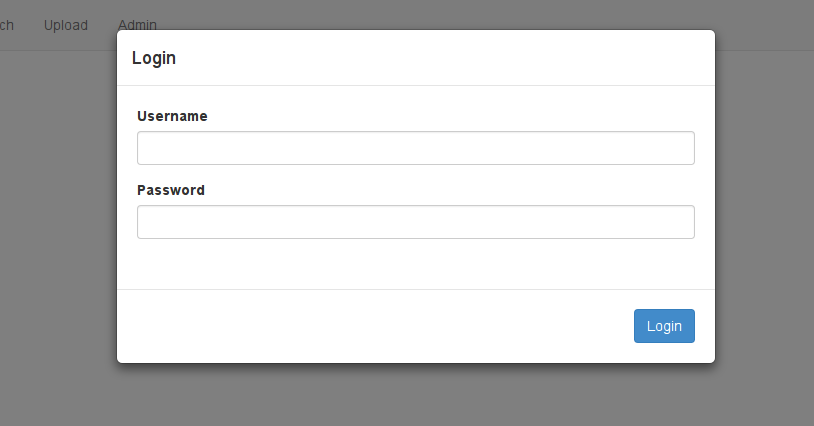
\includegraphics[width=0.75\textwidth]{web/manual/web_login.png}
\caption{\label{fig:web_search_login} The login pop-up window.}
\end{figure}
When first entering the web page, the login pop-up window in \refer{fig:web_search_login} is shown and the user will have to enter their username and password to gain access to the application.

%figure 2
\begin{figure}[h] 
\centering
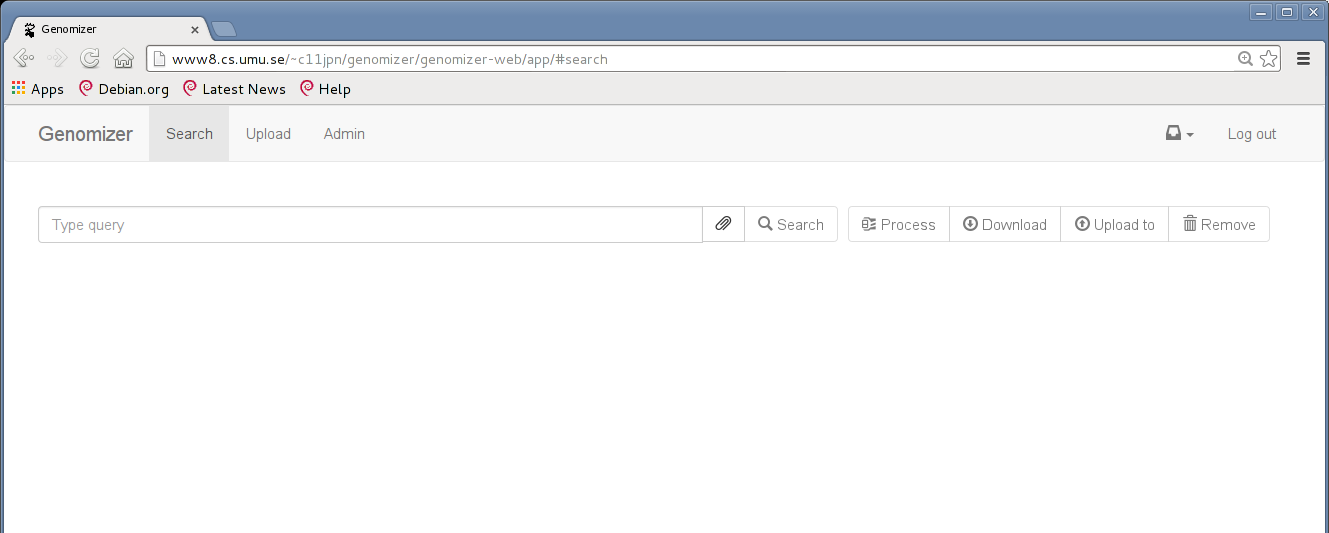
\includegraphics[width=1\textwidth]{web_search_welcome.png}
\caption{\label{fig:web_search_welcome} The start view of the web page.}
\end{figure}

When the user has logged in, the user is taken to the search page as shown in \refer{fig:web_search_welcome}.

The navigation bar at the top has a number of buttons to the left and two buttons to the right with the following functionality:
\begin{itemize}
	\item Clicking the “Genomizer” logo takes the user right back to the start view.
	\item The “Search” button will bring up the search view where the user can enter search strings to be sent to the server, and view search results.
	\item The “Upload” button will bring up the upload view where the user can select files to be uploaded and input annotation to a new experiment.
	\item The “Process” button will bring up the process view where the user can select an experiment to process.
	\item The “Administration” button will bring up the admin view where the user can handle genome releases and annotations.
    \item The inbox icon on the left side opens a dropdown list which displays the statuses of files currently being processed.
    \item The “Log out” button will log out the user.
\end{itemize}
This navigation bar is persistent through all sub pages and can easily be accessed.

\subsubsection{Search view}

In the search view, below the navigation bar, a “search-and-functionality” bar is visible. There is a search field and there are seven buttons that are explained below, starting with the left-most button: 

\begin{itemize}
	\item ”Query builder”, represented by a paperclip, brings up a query builder, shown in \refer{fig:web_search_queryBuilder}, that helps unexperienced users construct a valid query used for searching experiments. Just select a value in the three fields and press add. The correct pubmed-styled query will be shown in the search field and the three query fields will be reset so the user can add more things to search for in their query.
	\item “Search” searches for the query in the search field. 
	\item “Process” processes the selected files. This feature is demonstrated further in \refer{fig:web_process_modalView}.
    \item “Convert” converts the selected files. This feature is demonstrated further in section \ref{sssec:convertView}.
    \item “Upload to” opens the upload view with the selected experiments selected where the user can upload new files to an already existing experiment.
    \item “Remove” opens a new view where the files which are going to be deleted are presented along with a confirmation dialog that the user really wants to delete those files and experiments.
\end{itemize}

\begin{figure}[h]
\centering
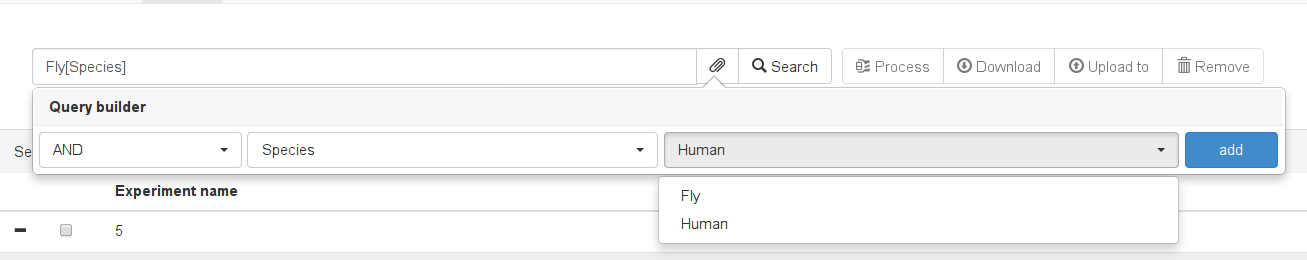
\includegraphics[width=1\textwidth]{web_search_queryBuilder.png}
\caption{\label{fig:web_search_queryBuilder}The query builder.}
\end{figure}

When first entering the search view, only the query builder button and the search button are clickable. The rest of the buttons become clickable once the user selects experiments or files. To search, the user can either write a pubmed style query (for example: \textit{”Fly[Species]”} to search for every experiment with ”Fly” as value of the annotation ”Species”) or use the query builder. When clicking the search button, a loading screen is shown. The experiment data is displayed once it has been retrieved from the server.

%figure x3
\begin{figure}[h]
\centering
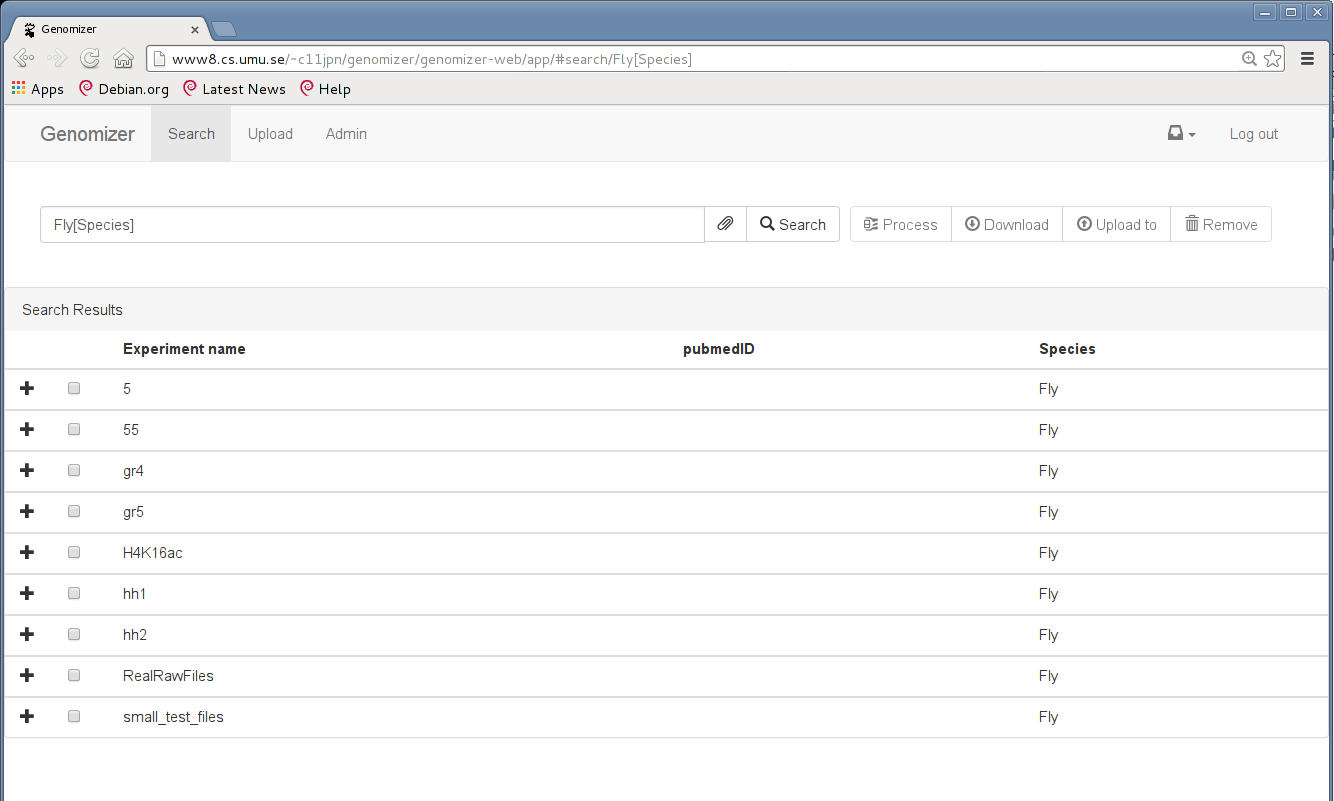
\includegraphics[width=1\textwidth]{web_search_searchTab.png}
\caption{\label{fig:web_search_searchTab}The search tab after searching for \textit{“Fly[Species]”}.}
\end{figure}

The view in \refer{fig:web_search_searchTab} is shown when the user has searched for the query \textit{”Fly[Species]”}. The displayed list contains all experiments returned from the search and a header on top with all annotation types. Every experiment can be expanded by clicking it to show the file types it contains. Each file type can be further expanded to show all files of that type in the experiment. Every file and experiment has a checkbox next to it that is used to select it. In \refer{fig:web_search_searchResult}, an experiment called \class{Ratiotest} and its contained collection of \class{raw} files have been expanded. Furthermore, the files \class{test.fastq} and \class{test2.fastq} have been selected. These files can now, for example, be processed or removed by using the buttons in the “search-and-functionality” bar.

%figure x4
\begin{figure}[h]
\centering
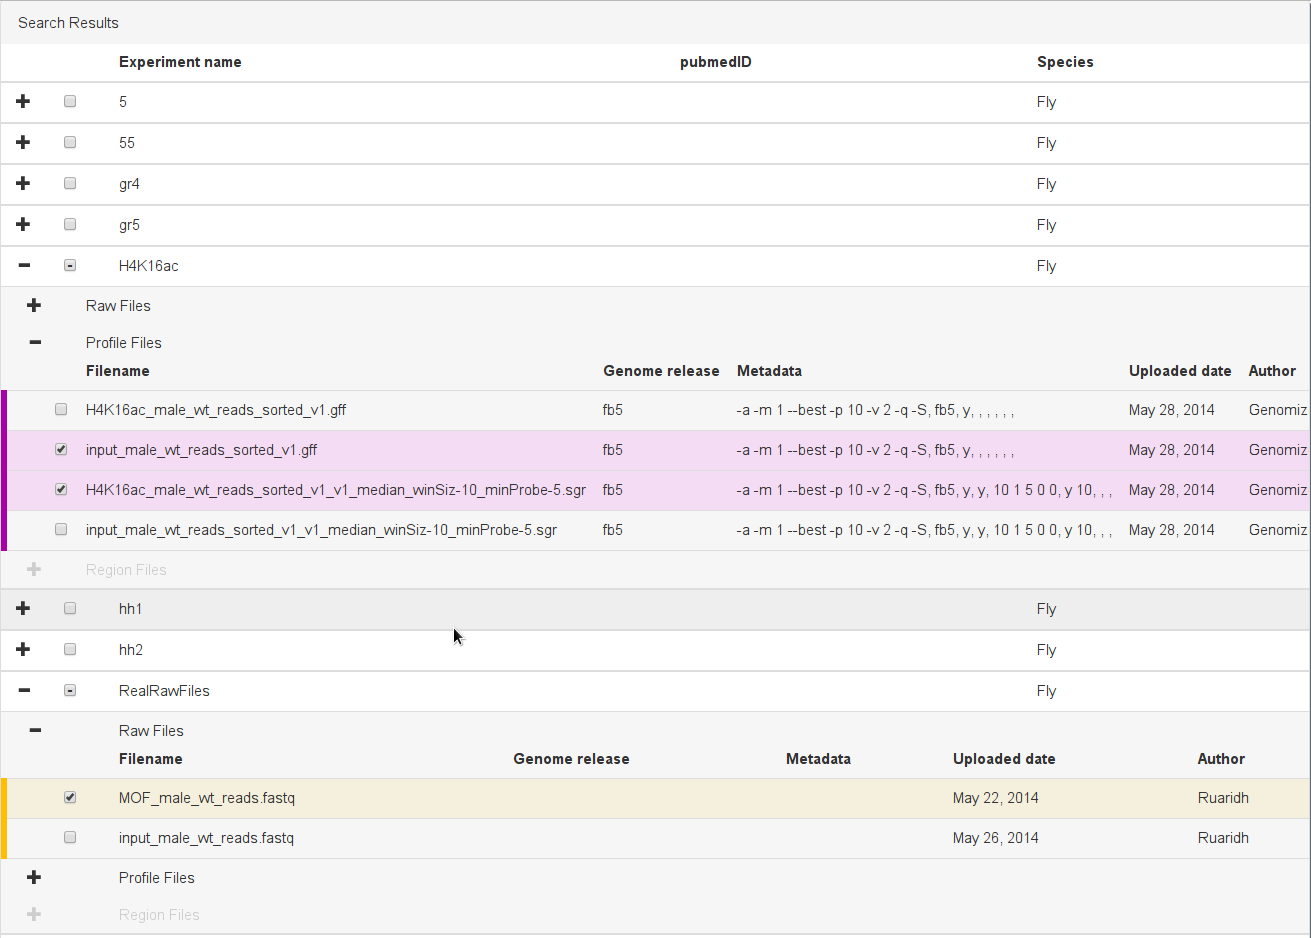
\includegraphics[width=1\textwidth]{web_search_searchResult.png}
\caption{\label{fig:web_search_searchResult}The search results table zoomed in, displaying the information of a \class{raw} file after having expanded an experiment.}
\end{figure}

If no experiments match the search query, the Search Results table will be empty stating “No search results found”.

\pagebreak
\subsubsection{The processing modal}
%figure X6
\begin{figure}[h]
\centering
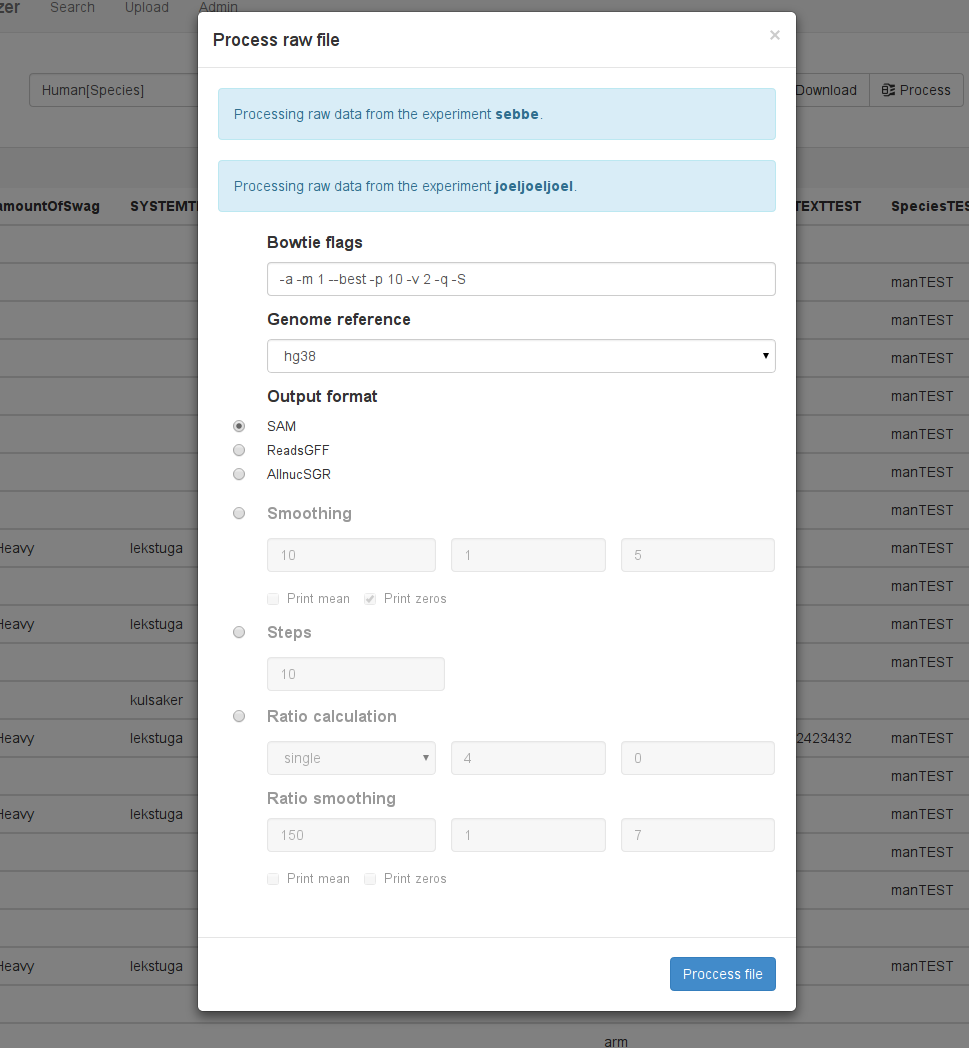
\includegraphics[width=1\textwidth]{web_process_modalView.png}
\caption{\label{fig:web_process_modalView}The processing modal.}
\end{figure}
\FloatBarrier
When the user has selected some files that are going to be processed the user will be presented with the view from \refer{fig:web_process_modalView}. The user can here choose which level of processing should be done on the \class{raw} files.

By clicking the radio buttons on the left side that much processing will be done on the \class{raw} files. All the steps above the selected will also be executed since they are needed to reach that level of processing.
At the top of the modal the experiments currently going through processing are presented.
\begin{figure}[h]
\centering
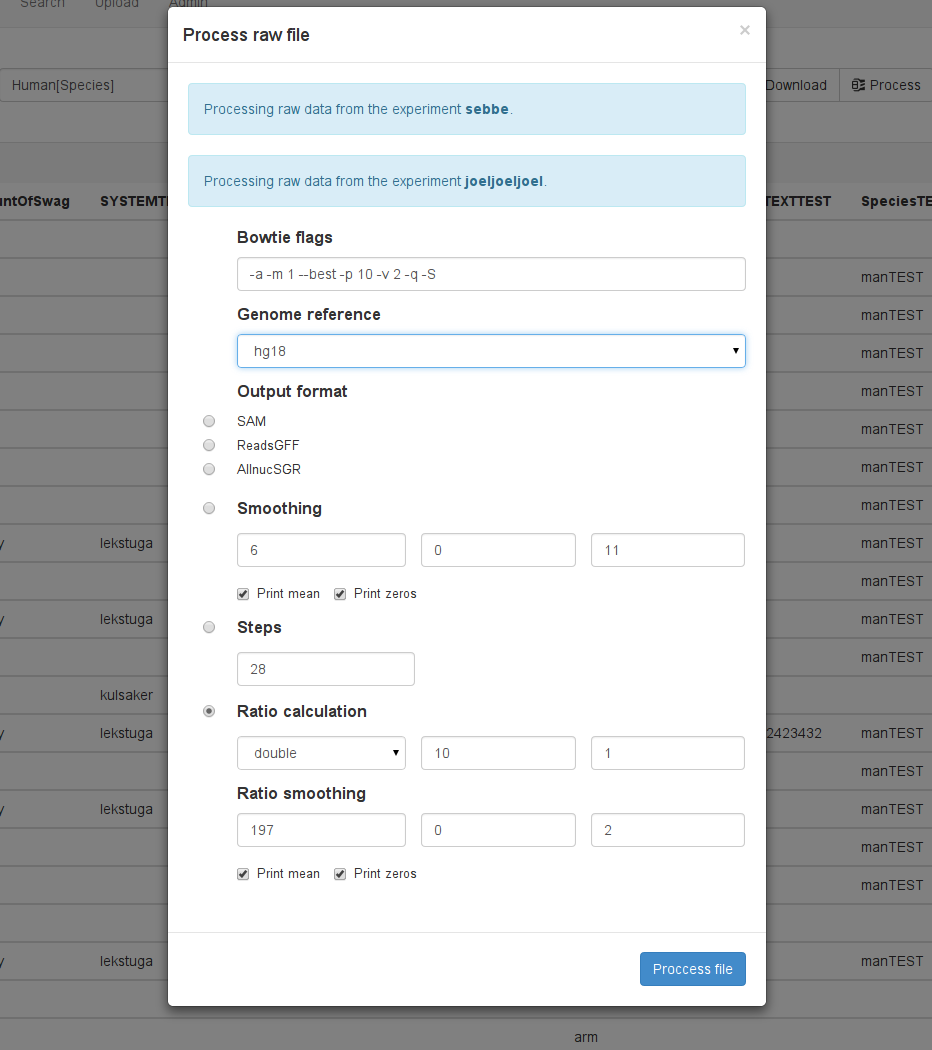
\includegraphics[width=1\textwidth]{web_process_modalValues.png}
\caption{\label{fig:web_process_modalValues}The process modal with selected parameters.}
\end{figure}
\FloatBarrier
When the user has decided the parameters as shown in \refer{fig:web_process_modalValues} and wants to start the processing the process button in the bottom right should be pressed. 
\begin{figure}[h]
\centering
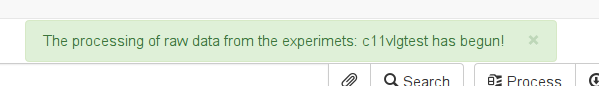
\includegraphics[width=0.8\textwidth]{web_process_success.png}
\caption{\label{fig:web_process_success}Success message.}
\end{figure}
\FloatBarrier
When results are received from the server and they were all successful the processing modal will disappear and a success message indicating that the processing is starting will be displayed to the user like in \refer{fig:web_process_success}.
\begin{figure}[h]
\centering
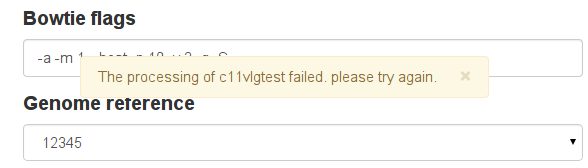
\includegraphics[width=0.8\textwidth]{web_process_notSuccess.png}
\caption{\label{fig:web_process_notSuccess}Fail message.}
\end{figure}
If some of the files that was going to be processed did for some reason fail the user will learn this by a warning message that tells the user which experiment did not start processing and which did as shown in \refer{fig:web_process_notSuccess}. The ones which started to process will be removed from the modal and the ones that did not start to process will remain. The user can now choose other parameters or do something else to make it work and try to submit a processing request again.
\pagebreak



\subsubsection{The convert view} \label{sssec:convertView}

The web application allows conversion between a number of file formats which both are of profile type. More specifically, the user may convert any of the file formats \class{.sgr, .wig, .bed} and \class{.gff} to either \class{.wig} or \class{.sgr}, with the exception that a file cannot be converted to the same file format.

\begin{figure}[h]
\centering
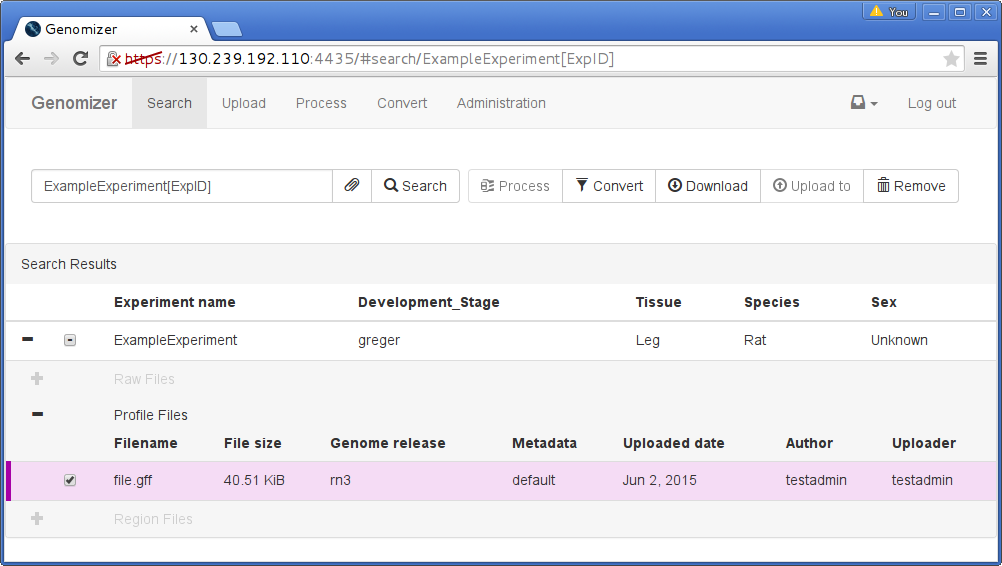
\includegraphics[width=1\textwidth]{web_convert_searchExp.png}
\caption{\label{fig:web_convert_searchExp}Selecting a file to convert.}
\end{figure}

Assume that there is an experiment \class{ExampleExperiment} which contains a profile file \class{file.gff}. Then the experiment will show up in the search view, see \refer{fig:web_convert_searchExp}, when typing ”ExampleExperiment[ExpID]” as search query and then clicking the search button. If the user wants to convert \class{file.gff} to a new file of format \class{.wig} called \class{file.wig}, the following steps can be taken:
\begin{itemize}
	\item From the view in \refer{fig:web_convert_searchExp}, select \class{file.gff} by clicking in its checkbox.
	\item Click the “Convert” button next to the search text field.
	\item The user will now be taken to the convert view shown in \refer{fig:web_convert_convertView}.
	\item Select \class{file.gff} by clicking on it.
	\item Mark the \class{.wig} checkbox in “Convert to” and click the “Convert” button.
\end{itemize}

\begin{figure}[h]
\centering
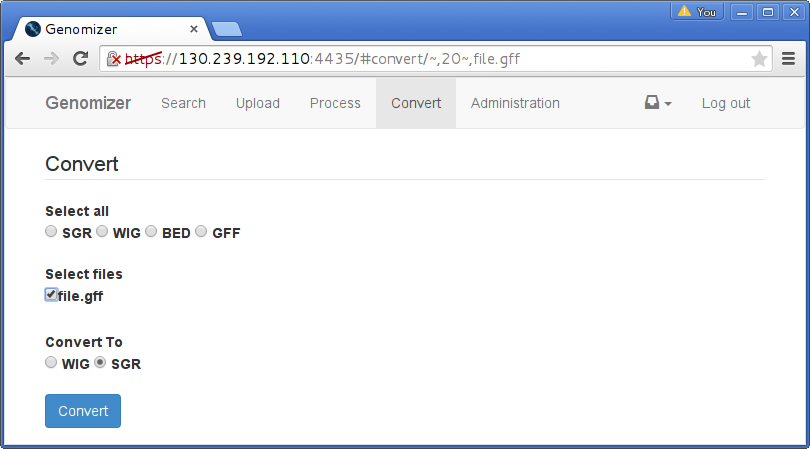
\includegraphics[width=1\textwidth]{web_convert_convertView.png}
\caption{\label{fig:web_convert_convertView}The convert view.}
\end{figure}

The file conversion will now start on the server. Once the conversion is done, the user will be able to see \class{file.wig} listed together with the old file \class{file.gff} when searching for the experiment.

If multiple files are selected for conversion, all of them will appear as a list in the convert view. If the user quickly wants to select all files of a specific file format, for example all \class{.wig} files, the GFF option can be marked in “Select all”. Then all files in the list of the format \class{.wig} will automatically be selected.

\subsubsection{The remove pop-up window}
\begin{figure}[h]
\centering
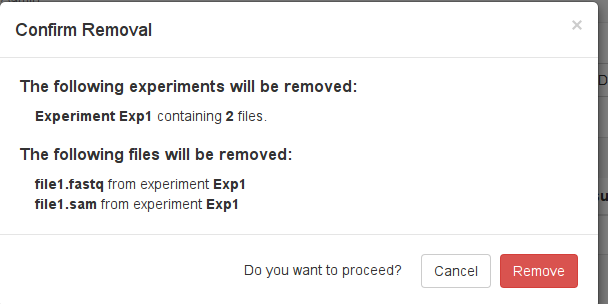
\includegraphics[width=0.8\textwidth]{web/manual/web_remove.png}
\caption{\label{fig:web_remove_removeFiles}The remove pop-up window.}
\end{figure}
\FloatBarrier
When the remove button is pressed the pop-up window in \refer{fig:web_remove_removeFiles} is shown displaying which files and experiments will be removed when the remove button is pressed.


\subsubsection{The process status dropdown}
\begin{figure}[h]
\centering
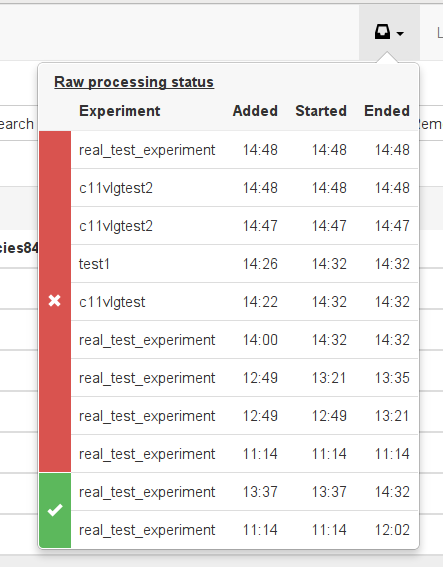
\includegraphics[width=0.5\textwidth]{web_processStatus_withData.png}
\caption{\label{fig:web_processStatus_withData}The process status dropdown.}
\end{figure}
\FloatBarrier
When pressing the inbox icon, a dropdown is shown as in \refer{fig:web_processStatus_withData} displaying the status of experiments currently being processed. There are four different statuses a processing can have, all grouped into colors: Waiting (yellow), Running (blue), Complete (green) and Failed (red). For example, in the figure, the two bottom experiments are complete and the rest have failed. If there are no experiments being processed, the dropdown will simply display “No process status available”.


\subsubsection{The upload view}

%figure X7
\begin{figure}[h]
\centering
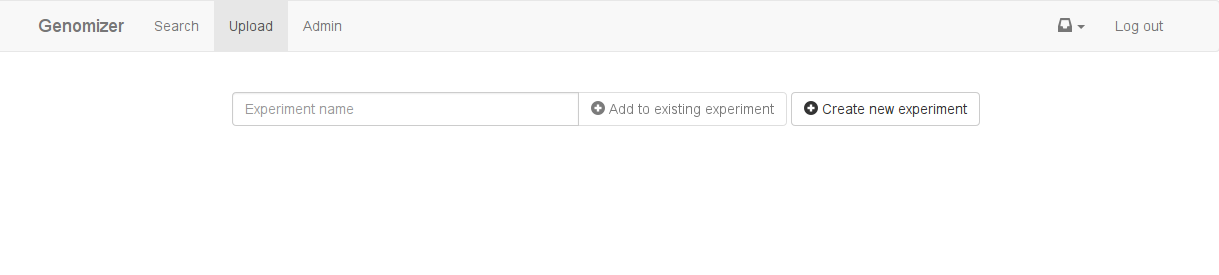
\includegraphics[width=1\textwidth]{web_upload_uploadView.png}
\caption{\label{fig:web_upload_uploadView}The upload view.}
\end{figure}

When the user clicks the upload tab in the navigation bar, the view in \refer{fig:web_upload_uploadView} will appear. The user has the option to create a new and fresh experiment or to load an existing experiment by entering its experiment name. 

%figure X8
\begin{figure}[h]
\centering
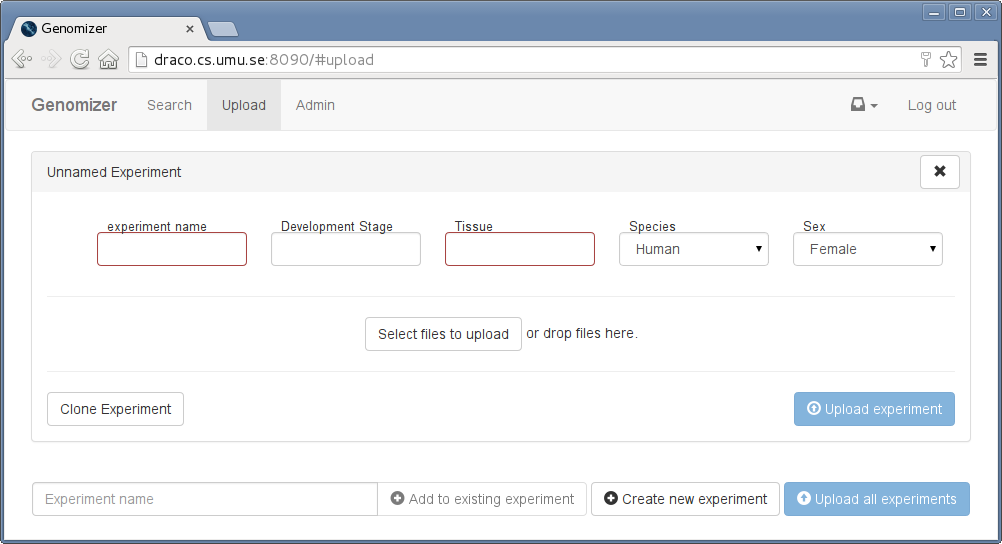
\includegraphics[width=1\textwidth]{web_upload_newExperiment.png}
\caption{\label{fig:web_upload_newExperiment}Creating a new experiment.}
\end{figure}

After clicking the “Create new experiment” button, the view in \refer{fig:web_upload_newExperiment} will appear. Here the user can input the annotations for the experiment through either freetext fields or dropdown lists. If a freetext field has a red border around it, that annotation is required and the experiment cannot be uploaded before all required fields have been filled in and at least one file has been added.

The user can create more experiments by clicking the “Create new experiment” button and a new empty experiment will be placed below the first experiment. The user can also clone an experiment by clicking the “Clone Experiment” button. What happens in this case, is that the every filled-in annotations gets copied to the new experiment.

To add files to the experiments the user can browse for local files and upload them by clicking the “Select files to upload” button. The user will only see file types that have to do with experiments but have the ability to search for all file types. There is also a way of adding files to the experiment by dragging them from a file browser and dropping them onto the experiment “drag and drop”.

An experiment can only contain two \class{raw} files and if the user tries to upload more a message with this information will appear and the experiment cannot be uploaded before the extra \class{raw} file/s is removed. 

To add files to a existing experiment the user types the name of the experiment in the field next to the “Upload to existing experiment” and clicks the button. If the experiment exists on the server it will appear in the experiment view the same way that a new experiment is shown. The annotations of an existing experiment cannot be changed from this view and if there are files already in this experiment they cannot be manipulated. Adding new files to existing experiments works the same way as to a new experiment.

%figure X9
\begin{figure}[h]
\centering
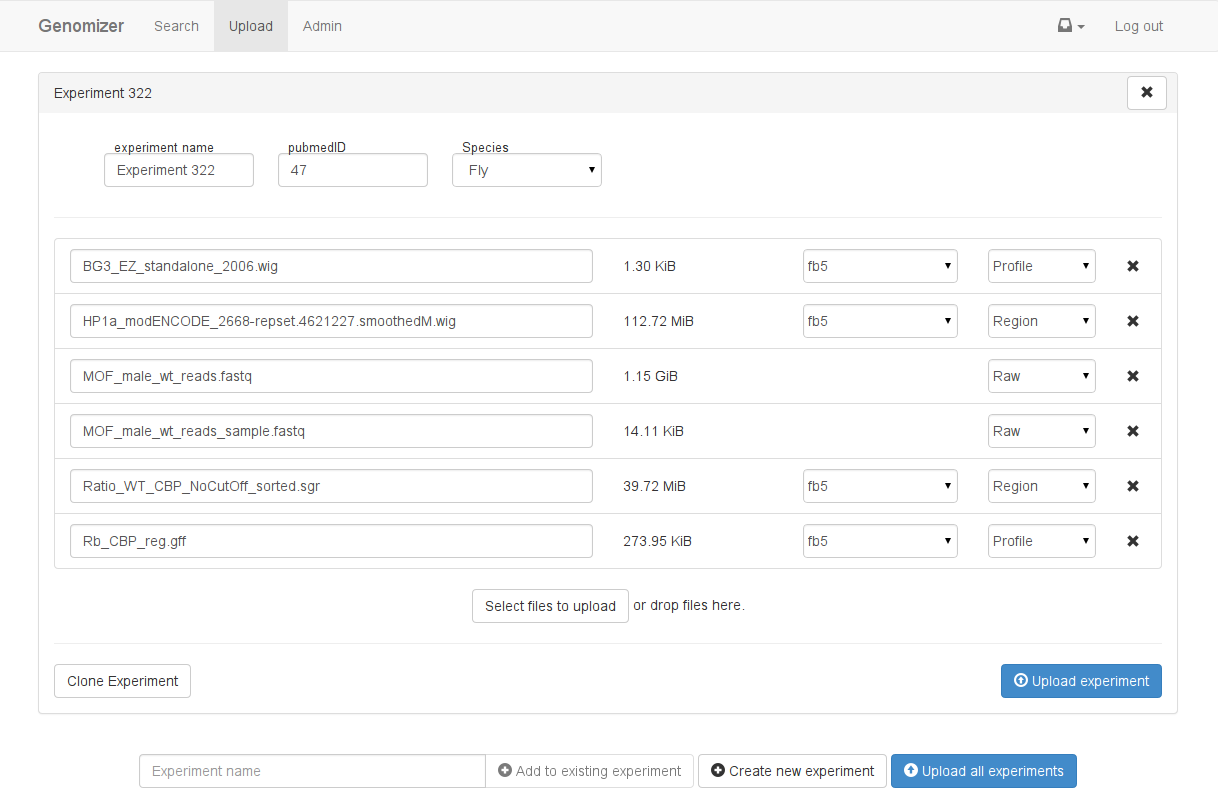
\includegraphics[width=1\textwidth]{web_upload_fileUpload.png}
\caption{\label{fig:web_upload_fileUpload}Files selected for upload.}
\end{figure}
 
When the user selects files, they will appear below the annotations as in \refer{fig:web_upload_fileUpload}. The file name is displayed in a text field on the left side of the file view. Next to the file name is a box that shows the size of the selected file. On the right side there is an option to select what type of file is being uploaded and an option to remove the file from the experiment. If the file type is either \class{profile} or \class{region}, there is an option to select what genome release the file is mapped to. The file type option will automatically be filled in with a guessed value depending on the file ending as follows: \class{.fastq} files are considered \class{raw} and all other formats (\class{.sgr, .wig, .gff}) are interpreted as \class{profile}.

When the user is done selecting files, filling in annotations and clicks the “Upload experiment” button the experiment view will be minimized showing only the name of the experiment and the progress bar of the files being uploaded. When the progress bar is done it turns green and now the experiment with all the files have been uploaded to the server. The user also has a way of uploading several experiments at the same time by clicking “Upload all experiments”. 

\subsubsection{System administration view}

This part of the web application is only accessible if the user has administrator rights. It is integrated with the rest of the web user interface and accessible through the “Administration” tab. The administrator can through this site see all annotations, add new annotations and edit existing ones.

The start page of this section has a “Create New Annotation” button, a list of existing annotations in the database and an edit button per existing annotation. The view looks like in \refer{adm__web_annotationView}. 

\begin{figure}[h]
 \addImage{web_SysadminAnnotationView.jpg}
 \caption{The start page for the administrator in the web client.}
 \label{adm__web_annotationView}
\end{figure}

For each annotation in the annotations list, an “Edit” button is available. When pressed, it will take the user to a page in which they can edit the selected annotation to change its name and what values the dropdown list will have if it is not a freetext field (see \refer{adm_web_editView}). 

\begin{figure}[h]
 \addImage{web_SysadminEditView.jpg}
 \caption{The edit annotation view.}
 \label{adm_web_editView}
\end{figure}
In the edit page, the admin can see the attributes of the chosen annotation and is able to delete the chosen annotation or change the information of it. The “Delete Annotation” button will delete the whole annotation, and for that reason two pop-up windows will appear to confirm that the administrator is sure of the action.

The administrator can change the list of annotation values. The site will automatically check whether something is added, removed or both and sends a request to change the annotation values to the server when the “Update Annotation” button is clicked.

If the admin clicks on the “Create new annotation” button from the admin start page, another view will open with the following structure:
\begin{itemize}
 \item Annotation Name
 \subitem Admin can enter a name for the annotation.
 
 \item Annotation Types
 \subitem Yes/No/Unknown - creates a dropdown list with those three options.
 \subitem freetext - creates an annotation where the users will be able to enter anything.
 \subitem Dropdown list - will enable a fourth field enabling the admin to enter which items that this list will contain.
 
 \item Forced Annotation
 \subitem Admin can choose if the new annotation should be required by users to enter. 
\end{itemize}

A Create Annotation will, if all necessary information has been entered, result in a popup (see \refer{adm_web_createPopup}) showing the resulting annotation and if confirmed, the annotation is added to the database. 
If canceled the administrator can keep making changes or go back to exit this view. If not all values is entered the admin will be alerted of the mistake and nothing will be created.

\begin{figure}[h]
 \centering
 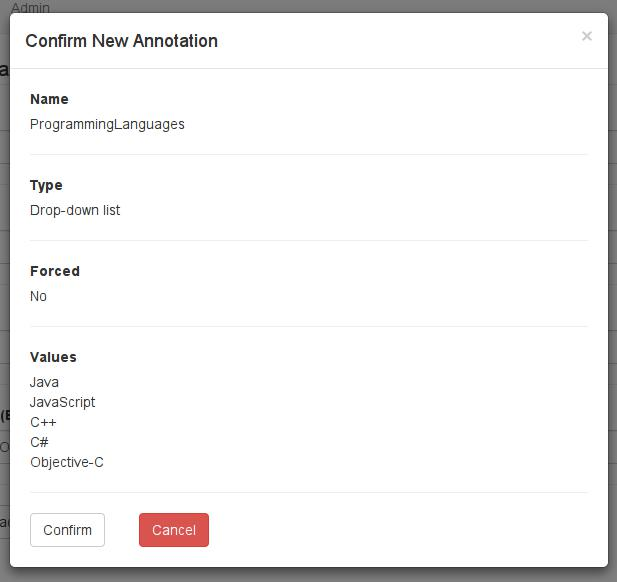
\includegraphics[width=0.7\textwidth]{web_SysadminCreateAnnotationConfirm.jpg}
 \caption{The confirm annotation pop-up.}
 \label{adm_web_createPopup}
\end{figure}



The example in \refer{adm_web_createPopup} will result in a drop-down annotation with the name Number of toes and possible values: 0, 1, 2, 3, 4, 5 with 0 as default and is not forced.

A back button which takes the user back to the annotations start page is also available in this view. In \refer{adm_web_createView} the create annotation view can be seen.

\begin{figure}[t]
 \addImage{web_SysadminCreateAnnotation.jpg}
 \caption{The view for administrators where new annotations can be created.}
 \label{adm_web_createView}
\end{figure}

The “Genome-releases” link on the sidebar takes the administrator to a page where it is possible to add and remove genome releases to and from the server (see \refer{adm_web_genomereleaseView}.

\begin{figure}[h]
 \addImage{web_SysadminGenomeReleaseView.jpg}
 \caption{The genome-release view.}
 \label{adm_web_genomereleaseView}
\end{figure}

The button “Select files to upload” opens the native file explorer where the user can select one ore multiple files and click on “OK”. This will open a popup-window, seen in \refer{adm_web_uploadconfirm}, showing what files that where chosen and asks for species and genome version before uploading. 

\begin{figure}[h]
 \centering
 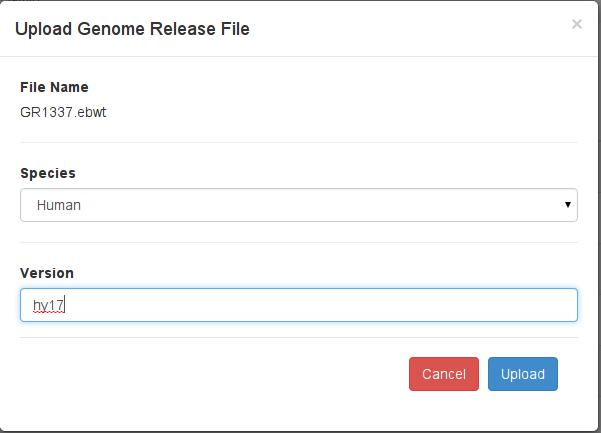
\includegraphics[width=0.7\textwidth]{web_SysadminUploadGenomeReleaseModal.jpg}
 \caption{Popup for uploading genome releases.}
 \label{adm_web_uploadconfirm}
\end{figure}

When the upload begins the popup closes and a progress-bar appears showing the progress, showing ''Upload completed'' when done. The user can at this stage move between pages without disturbing the upload but should not close or refresh the web browser. 

Every genome release in the table can be deleted by clicking on the “Delete” button next to the release. This will prompt a small popup asking for user confirmation and if given a positive response, deletes the genome release from the server and updates the view. 

If any genome release is used by an experiment already an error will appear telling the user exactly that. 

\subsection{Setting up the application}
To setup the application, move the content of the folder \url{genomizer-web/app/} to the desired location from where the application should be run. To run the web page, open a web browser and enter the url to the folder which contains the \class{index.html} file (where the content of app was placed).
For example, given that the \url{genomizer-web} folder is placed in the home folder of the Umeå university CS user \class{c12abc} and that user wants to put the web app in a folder called \url{public/html/} which is also in the home folder of the user. In Linux, do the following steps:
\begin{enumerate}
	\item Navigate to the app folder: \texttt{“cd ~/genomizer-web/app/”}
	\item Move the contents of app to the folder \url{public/html}: \texttt{“mv * ~/public\_html/”}
	\item Given that the url to \url{public/html} is: \filePath{“www8.cs.umu.se/~c12abc/”}
	\item To run the application start a web browser and type \filePath{“www8.cs.umu.se/~c12abc/”}
\end{enumerate}
This will open the web page in the browser.



\chapter{Android manual}
In this section instructions for the usage of the \appName\ Android application is presented. In \refer{sec:and_start} there is a description on how to start the application and \refer{sec:and_search} gives instructions on how to search for experiments.

\subsection{Start the Application and Login}
\label{sec:and_start}

%Localize the \appName\ icon in your list of Android applications and click the icon in order to start \appName.

The user needs to login in order to start working with the \appName\ app. The  user name and password is inserted in the corresponding boxes and the clicking the \term{Sign in} button initiates the main application. If you dont have a user name or password, the system administrator should be contacted to help with the creation of an account.

\begin{figure}[h]
\addScaledImage{0.1}{figures/and_login.png}
\caption{Login View}
\label{fig:and_login_man}
\end{figure}
\FloatBarrier


In \refer{fig:and_login_man}, the tool button in the upper right corner leads to the \term{Settings View}, described in  \refer{sec:and_manual_settings} below.

\subsection{Settings}\label{sec:and_manual_settings}
The \term{Settings} view acts to enable the user to choose which server to connect to when using the Genomizer application. As of the current release of the application, in the Settings View, the user is able to:

\begin{enumerate}
\item Select one of previously used server URLs
\item Add a server URL
\item Remove a server URL
\item Edit an existing server URL
\end{enumerate}

The left most image in \refer{fig:and_settings_man} show three buttons in the top right corner of the view. These buttons are used to access the functionalities listed above. The button with a green plus sign enables the user to add a new server URL, as illustrated in the image in the middle of \refer{fig:and_settings_man}. The button in the middle with a paint brush icon will on selection show the server URL edit view, as illustrated in the right most image in \refer{fig:and_settings_man}. And the left most button with a red cross icon will upon selection enable the user to remove the currently selected server URL from the drop down menu containing all saved server URLs.


Any selection, removal, edit or addition of server URLs are stored locally on the device and and are loaded upon subsequent application launches.


\begin{figure}[h]
\addThreeImages
{figures/and_server_settings_select.png}
{figures/and_server_settings_add.png}
{figures/and_server_settings_edit.png}
\caption{Settings View}
\label{fig:and_settings_man}
\end{figure}
\FloatBarrier


\subsection{Searching for files}\label{sec:and_search}

When entering the Search View, as illustrated in \refer{fig:and_search_man} all annotations are automatically downloaded from the server and displayed as a list. Each annotation consists of an annotation-identifier, a dropdown table/text-input field where the user may specify desired value, and a checkbox. When putting a check-mark in the checkbox, it means that this particular annotation type should be used when searching for files in the database. The search is initiated by pressing \term{Search} at the bottom of the view.

Once the user has been logged in to the system, three buttons will always be visible in the top right corner of each view:
\begin{enumerate}
\item Search button
\item Selected Files button
\item Process Status button
\end{enumerate}

Clicking these buttons switches the context of the application and allow the user to quickly navigate between different functionalities.

The search view also contain a button visible in the top right corner, used to activate the advanced search mode described in the following \refer{sec:and_search_pub}. 

\begin{figure}[h]
\addScaledImage{0.1}{figures/and_search.png}
\caption{The Search View}
\label{fig:and_search_man}
\end{figure}
\FloatBarrier


\subsection{Pubmed Search}\label{sec:and_search_pub}
The Pubmed Search view provide the means of free-text search using Pubmed-Style queries as seen in \refer{fig:and_pubmed_man}. This view include a text-input field together with two buttons. The text field  is populated with the annotations that the user may have selected within the regular Sarch View. However, if no annotations have been previously selected in the Search View, the user must input all annotations manually. The annotations selected in the Search View are associated with logical connectives. These logical connectives, as well as annotation values, can be manually modified by the user. The supported logical connectives are: 

\begin{enumerate}
\item AND
\item NOT
\item OR
\end{enumerate}

The user may also choose to provide perentheses to device more specific searches.

\begin{figure}[h]
\addScaledImage{0.1}{figures/and_search_advanced.png}
\caption{The Pubmed Search View}
\label{fig:and_pubmed_man} 
\end{figure}
\FloatBarrier


%Explains several steps, remove others or shorten this?
\subsection{Search Results}
When searching the user will be redirected to the search results view  that displays a list of available experiments matching the search annotations. Every experiment is listed showing the experiment name. To receive more information about data files that are available for each experiment, click on an experiment in the list. By clicking an entry you will be taken to a new view displaying all available data files for that experiment, presented in the Experiment List View. 

Clicking on the cogwheel button in the top right corner of the view enables the user to modify which annotations are presented within the Search Results View, and is described further in the following \refer{sec:search_settings}.

\begin{figure}[h]
\addScaledImage{0.1}{figures/and_search_result.png}
\caption{The Search Results View}
\label{fig:and_search_results_man} 
\end{figure}
\FloatBarrier


\subsection{Search Settings View}\label{sec:search_settings}
The Search Settings View display settings for the files presented to the user after a search is done, as illustrated in  \refer{fig:and_search_settings_man} below. The Search Settings View contains all different annotations the user will be able to display about the experiments presented in the Search Results View. The user are able to select annotations by marking the checkbox next to the annotation name and then clicking the Save settings button to save changes. If the user has no special requests it is also possible to use default settings, which will display (experiment-Id, created by, pubmed and type) annotations for the files displayed. 



\begin{figure}[ht]
\addScaledImage{0.1}{figures/and_search_select_visible_annotations.png} 
\caption{Search Settings View}
\label{fig:and_search_settings_man}
\end{figure}
\FloatBarrier


\subsection{Experiment File View}
The Experiment File View is used to present the user with all files associated with an experiment. This includes all raw, profile and region files derived from the experiment. A user may select and add an arbitrary number of files to the Selected Files view, which is described in \refer{sec:and_manual_selected}, by marking the checkbox of the desired files, as done in  \refer{fig:and_experiment_man}, and pressing \term{Add to selection}.

Clicking on a file presented within this view creates a popup containing all different annotations for the selected file, as illustrated in the right most image in \refer{fig:and_experiment_man}.

\begin{figure}[h]
\addTwoImages{figures/and_experiment_files.png}{figures/and_experiment_file_info.png}
\caption{The Experiment File View}
\label{fig:and_experiment_man}
\end{figure}
\FloatBarrier






\subsection{Selected Files}\label{sec:and_manual_selected}
Once the user has signed in to the server, the user is presented with a \term{Selected Files} view, as illustrated in \refer{fig:and_selected_man}.
This is the main part of the application where all work and conversions are done to files, when the user has searched and found files that are interesting for further use, it can be moved to the selected files area. 
The page contains three different tabs that the user may use to show different type of files saved in the selected files workarea. All files stored in this page are only saved during the current session and is meant to be used as a temporary grouping area for files. 

\begin{itemize}

	\item \term{Raw}, will diplay all the Raw files that the user has choosen to save to the temporary work area. The files here can be marked and used for converting to profile data.
    \item \term{Profile}, will display the Profile files that the user has choosen to move to the selected files area. No conversions or other work can be done at this stage to profile files.
    \item \term{Region}, this page will display all the region files the user has selected to move to the selected files area for further work. No conversions or other work can in this stage be done to region files.
    
\end{itemize}

Similar to the Experiment View, clicking on a file will present the user with a popup containing the annotations for that file.


\begin{figure}[h]
\addTwoImages{figures/and_selected_files.png}{figures/and_selected_files_file_info.png}
\caption{Selected Files View}
\label{fig:and_selected_man}
\end{figure}
\FloatBarrier


\subsection{Converting Files}
When the user has choosen a file (or several files) for conversion, the user will be presented with the Conversion View as seen in \refer{fig:and_conversion_man}. In this view the user may enter the parameters needed to perform a Raw-to-Profile-file conversion.
\newline
There are 9 different parameters to be specified in this page for the conversion to be done in a proper way. All parameters do not have to be filled, but they have to be specified in the order that is presented to the user. In order to fill out parameter number 3, both parameter 1 and 2 have to be filled out first.

\begin{enumerate}
	\item \term{Bowtie}, is a freetext field where the different parameters for the bowtie program are to be inserted.
    \item \term{Genome Version}, is a dropdown menu where the user is presented with all the different genome versions that can be used for the conversion.
    \item \term{Sam to GFF}, is an on/off option.
    \item \term{GFF to SGR}, is an on/off option. 
    \item \term{Smoothing}, free text field for the parameters for smoothing if it is to be used.
    \item \term{Stepsize}, free text field for which stepsize is to be used for the conversion.
    \item \term{Ratio calculation}, on/off field which determines if the ratio calculation is to be used. If checked it will require both next two fields to be filled out.
    \item \term{Ratio}, free text field with the parameters for the ratio, if ratio calculation is wanted.
    \item \term{Smoothing}, free text field for parameters regarding the smoothing for the ratio calculation.     

\end{enumerate}

\begin{figure}[h]
\addScaledImage{0.1}{figures/and_convert_view.png}
\caption{The Conversion View}
\label{fig:and_conversion_man}
\end{figure}

\FloatBarrier


\subsection{Process View}
The process view, as illustrated in \refer{fig:and_process_man} below, is used to visualize the current workload on the server. The view contains a list of tasks that has been assigned to the server. Each task contains the name of the experiment in which the process is currently operating in, the time when the process was added, the time when the process was started and the time when the process was finished. Each item also contains information about the process current state.

Each process may have one of these four states:
\begin{enumerate}
\item{Waiting} - The task is awaiting processing by the server
\item{Started} - The task is currently being processed by the server
\item{Finished} - The task has been completed
\item{Crashed} - The task was not successfully completed
\end{enumerate}

\begin{figure}[h]
\addScaledImage{0.1}{figures/and_process_status.png}
\caption{ The Process View}
\label{fig:and_process_man}
\end{figure}

\FloatBarrier


\chapter{iOS manual}
\subsection{How to run the app in Xcode}
In order to use the program, import the project from github into Xcode from the following repository:
\url{https://github.com/genomizer/genomizer-iOS.git} 

To compile and run the program, press \click{cmd+R}. A simulator will start and the login screen will be shown as seen in \refer{fig:ios_login}a.

\subsection{How to login}

\begin{enumerate}
\item Tap the settings button in the upper right corner and enter the url and port for the server you want to use and press \click{Done}. See \refer{fig:ios_login}a,c.
\item Tap on the \click{Username} textfield and enter your username.
\item Tap on the \click{Password} textfield and enter your password.
\item Tap on \click{Sign in} to sign in.
\end{enumerate}
A user gets logged in when accepted credentials are entered in the ‘username’ and ‘password’ fields and the ‘Sign in’ button is pressed. If incorrect credentials are entered, a popup message is shown, informing the user that the username or password is incorrect.

\begin{figure}[ht]
\addThreeImages{ios_login1.PNG}{a}{ios_login2.PNG}{b}{ios_login3.PNG}{c}
\caption{The login screen.}
\label{fig:ios_login}
\end{figure}
\FloatBarrier

\subsection{How to logout}
\begin{enumerate}
\item Tap \click{Gear}-symbol on the tab bar and a \emph{Setting}-screen will appear. See \refer{fig:ios_more}
\item Tap \click{Logout} to logout.
\end{enumerate}

\begin{figure}[htb]
\addScaledImage{0.17}{ios_settings.PNG}
\caption{The settings screen.}
\label{fig:ios_more}
\end{figure}
\FloatBarrier

\subsection{How to search for experiments}

\begin{enumerate}
\item Ensure that you on the search-screen by looking at the title on the top. If it says \emph{Search} you can skip step (2). 
\item Tap on leftmost button(magnifying glass) on the tab bar which you can find on the bottom of the screen.
\item Tap on the annotation you want to search for and a spinning wheel with options will appear from the bottom of the screen. See \refer{fig:ios_search}a.
\item Drag the wheel up or down to select the option you want.
\item Enable the annotation to use when searching by toggling the switch to the right of the annotation. See \refer{fig:ios_search}b.
\item Do steps (2)-(4) for more search criteria.
\item Tap \click{Search} to search.
\end{enumerate}

\begin{figure}[ht]
\addThreeImages{ios_search1.PNG}{a}{ios_search2.PNG}{b}{ios_search4.PNG}{c}
\caption{The search screen.}
\label{fig:ios_search}
\end{figure}
\FloatBarrier

\subsection{How to use advanced search}

\begin{enumerate}
\item Ensure that you on the search-screen by looking at the title on the top. If it says \emph{Search} you can skip step (2). 
\item Tap on leftmost button(magnifying glass) on the tab bar which you can find on the bottom of the screen.
\item Tap on the symbol to top right of the screen and a new view will appear with the title \emph{Advanced Search}. See \refer{fig:ios_search}c.
\item Write your search criteria in PubMed-style and tap \click{search}
\end{enumerate}
The annotations you select on the search-screen will also show in advanced search.

\subsection{How to process files}


\begin{enumerate}
\item Search for experiments
\item In \emph{Search Results}-screen tap on an experiment and the \emph{Files}-screen will appear showing the files which belongs to the experiment. See \refer{fig:ios_files_view}a
\item Tap the \click{Plus}-symbol next to the file you want to process.
\item Do step (3) for every file you want to process. Same file can be used more than once. A counter will appear next to the Plus-symbol to keep track on how many times the file will be used in the process-step, see \refer{fig:ios_files_view}b.
\item Tap the \click{Process}-button and \emph{Make a process}-view will appear with every file you have selected. See \refer{fig:ios_make_process_view}a
\item Tap \click{Add Process} and select what kind of process you want to do on the selected files.
\item After you have selected a process the input files and output files will appear with the selected process separating them. You can add parameter values by tapping \click{Flag}-symbol below the input files. The output files can be renamed by tapping on the filename. See \refer{fig:ios_make_process_view}b
\item Do step (6) to create a sequence of processes to be made on the selected files. See \refer{fig:ios_make_process_view}c for an example of a process sequence.

\item Tap \click{Done}-button to send the sequence of processes to the server.
\end{enumerate}

%\begin{figure}[htb]
%\addScaledImage{0.17}{ios_process_files.jpg}
%\caption{Files screen.}
%\label{fig:ios_process_files}
%\end{figure}
%\FloatBarrier

\begin{figure}[htb]
\addTwoImages{ios_process_files.jpg}{a}{ios_files_added.jpg}{b}
\caption{Files view.}
\label{fig:ios_files_view}
\end{figure}
\FloatBarrier

\begin{figure}[htb]
\addThreeImages{ios_empty_make_process.jpg}{a}{ios_one_process.jpg}{b}{ios_many_process.jpg}{c}
\caption{Create processes.}
\label{fig:ios_make_process_view}
\end{figure}
\FloatBarrier


\subsection{How to set which annotation to be visible on Search Results}

\begin{enumerate}
\item In Search Results view, tap \click{Edit} and \emph{Select Annotations}-screen will appear
\item Select which annotations to show by toggle the switch next to each annotation.
\item Tap \click{Back} to go back to \emph{Search Results}. See \refer{fig:ios_searchResult}a-c
\end{enumerate}

\begin{figure}[ht]
\addThreeImages{ios_result1.PNG}{a}{ios_result2.PNG}{b}{ios_result3.PNG}{c}
\caption{Select annotation}
\label{fig:ios_searchResult}
\end{figure}
\FloatBarrier

%\subsection{How to remove files from workspace}
%\begin{enumerate}
%\item Tap \click{Star}-symbol on the tab bar to view the workspace.
%\item Toggle the switch next to the file you want to remove.
%\item Tap \click{Trash can}-symbol to the upper right corner to remove the selected files. See \refer{fig:ios_selectedFiles}
%\end{enumerate}

\subsection{How to view process status on the server}

\begin{enumerate}
\item Tap \click{Process}-symbol(the symbol between the star and the trash can) to view the processes on the server.
\item To refresh the view, drag the view down until an activity indicator icon is visible below the title of the screen and release. See \refer{fig:ios_processes}
\end{enumerate}

\begin{figure}[htb]
\addScaledImage{0.3}{ios_processes1.PNG}
\caption{The select task screen.}
\label{fig:ios_processes}
\end{figure}
\FloatBarrier

\subsection{How to view information about a file}

\begin{enumerate}
\item Tap \click{information}-symbol next to the file to view information of the file.
\item Close by tapping \click{Close}. See \refer{fig:ios_files1}a-b
\end{enumerate}

\begin{figure}[htb]
\addTwoImages{ios_files4.PNG}{a}{ios_files2.PNG}{b}
\caption{The files screen.}
\label{fig:ios_files1}
\end{figure}
\FloatBarrier






\end{document}
